%Jennifer Pan, August 2011

\documentclass[10pt,letter]{article}
	% basic article document class
	% use percent signs to make comments to yourself -- they will not show up.

\usepackage{amsmath}
\usepackage{amssymb}
	% packages that allow mathematical formatting

\usepackage{graphicx}
	% package that allows you to include graphics
\usepackage{tikz}
\usepackage{setspace}
	% package that allows you to change spacing

\onehalfspacing
	% text become 1.5 spaced

\usepackage{fullpage}
	% package that specifies normal margins

\renewcommand{\vector}[1]{\boldsymbol{#1}}
\newcommand{\problem}[1]{\section*{Problem #1}}
\newcommand{\problempart}[1]{\paragraph{#1}}

\begin{document}
	% line of code telling latex that your document is beginning


\title{ECON 511 Problem Set 2}

\author{Nicholas Wu}

\date{Spring 2021}
	% Note: when you omit this command, the current dateis automatically included

\maketitle
	% tells latex to follow your header (e.g., title, author) commands.
%\textbf{Note:} I use bold symbols to denote vectors and nonbolded symbols to denote scalars. I primarily use vector notation to shorthand some of the sums, since many of the sums are dot products.

\problem{1}
The maximization Hamiltonian is
\[ H = \pi(k_t, x_t)  - p^k_t I_t - p^k_t I_t D(I_t, k_t) + \lambda_t (I_t - \delta k_t)\]
The maximization conditions are:
\[ \lambda_t = p^k_t + p^k_t I_t D_I(I_t, k_t) + p^k_t D(I_t, k_t)  \]
\[ \pi_k(k_t, x_t) - p^k_t I_t D_k(I_t, k_t) - \delta \lambda_t = -\dot{\lambda_t} + r \lambda_t \]
\[ \lim_{t \to \infty} \lambda_t e^{-rt}k_t = 0 \]
Rearranging, we have
\[ \dot{\lambda_t} - r \lambda_t = \delta \lambda_t - \pi_k(k_t, x_t) + p^k_t I_t D_k(I_t, k_t)\]
Using the hint, we consider
\[ e^{rt} \frac{d}{dt}[\lambda_t k_t e^{-rt}]  \]
By the product rule
\[ e^{rt} \frac{d}{dt}[\lambda_t k_t e^{-rt}] =  e^{rt} \left( \dot{\lambda_t}k_t e^{-rt} + \lambda_t\dot{k_t}e^{-rt} - r\lambda_t k_t e^{-rt} \right) \]
\[ = \dot{\lambda_t} k_t + \lambda_t \dot{k_t} - r \lambda_t k_t \]
\[ = (\dot{\lambda_t} - r \lambda_t) k_t + \lambda_t \dot{k_t} \]
Plugging in what we know from maximization problem, we have
\[ = (\delta \lambda_t - \pi_k(k_t, x_t) + p^k_t I_t D_k(I_t, k_t))k_t + \lambda_t (I_t - \delta k_t) \]
\[ = (- \pi_k(k_t, x_t) + p^k_t I_t D_k(I_t, k_t))k_t + \lambda_t I_t \]
\[ = - k_t \pi_k(k_t, x_t) + k_t p^k_t I_t D_k(I_t, k_t) + (p^k_t + p^k_t I_t D_I(I_t, k_t) + p^k_t D(I_t, k_t)) I_t \]
\[ = - k_t \pi_k(k_t, x_t) + p^k_t I_t (k_t D_k(I_t, k_t) + 1 + I_tD_I(I_t, k_t) + D(I_t, k_t)) \]
Multiplying both sides by $e^{-rt}$ we get
\[ \frac{d}{dt}[\lambda_t k_t e^{-rt}] = \left(- k_t \pi_k(k_t, x_t) + p^k_t I_t (k_t D_k(I_t, k_t) + 1 + I_tD_I(I_t, k_t) + D(I_t, k_t)) \right) e^{-rt} \]
Integrating from 0 to $\infty$ and using transversality, we get
\[ - \lambda_0 k_0 = \int_0^\infty \left(- k_t \pi_k(k_t, x_t) + p^k_t I_t (k_t D_k(I_t, k_t) + 1 + I_t D_I(I_t, k_t) + D(I_t, k_t)) \right) e^{-rt} \ dt \]
\[ \lambda_0 k_0 = \int_0^\infty \left(k_t \pi_k(k_t, x_t) - p^k_t I_t (k_t D_k(I_t, k_t) + 1 + I_tD_I(I_t, k_t) + D(I_t, k_t)) \right) e^{-rt} \ dt \]
Then we have marginal $q$ at time zero is
\[ q_0 = \frac{\lambda_0}{p^k_0} = \frac{\int_0^\infty \left(k_t \pi_k(k_t, x_t) - p^k_t I_t (k_t D_k(I_t, k_t) + 1 + I_tD_I(I_t, k_t) + D(I_t, k_t)) \right) e^{-rt} \ dt}{p^k_0 k_0} \]
Average $Q$ is given by
\[ Q_0 = \frac{V_0}{p^k_0 k_0} = \frac{\int_0^\infty (\pi(k_t, x_t) - p^k_t I_t - p^k_t I_t D(I_t, k_t)) e^{-rt} \ dt}{p^k_0 k_0} \]
We want to find the conditions when $q_0 = Q_0$. Obviously, if the integrands are equal, $q_0 = Q_0$. Hence, the forward direction is clear. If the firm satisfies (i), (ii), and (iii), then the integrand of $q_0$ is
\[\left(k_t \pi_k(k_t, x_t) - p^k_t I_t (k_t D_k(I_t, k_t) + 1 + I_tD_I(I_t, k_t) + D(I_t, k_t)) \right) e^{-rt} \]
From (i) and (ii), we get $k_t \pi_k(k_t, x_t) = \pi(k_t, x_t)$,
\[ = \left( \pi(k_t, x_t) - p^k_t I_t (k_t D_k(I_t, k_t) + 1 + I_tD_I(I_t, k_t) + D(I_t, k_t)) \right) e^{-rt} \]
\[ = \left( \pi(k_t, x_t) - p^k_t I_t - p^k_t I_t (k_t D_k(I_t, k_t) + I_tD_I(I_t, k_t) + D(I_t, k_t)) \right) e^{-rt} \]
By (iii) and Euler's theorem, we get that $k_t D_k(I_t, k_t) + I_t D_I(I_t, k_t) = 0$, so
\[ = \left( \pi(k_t, x_t) - p^k_t I_t - p^k_t I_t  D(I_t, k_t) \right) e^{-rt} \]
Hence (i), (ii), and (iii) imply $q_0 = Q_0$.

For the converse, we need to show that if $q_0 = Q_0$, then the conditions (i)-(iii) must hold. Since $q_0 = Q_0$, we must have that this holds regardless of choice of $k_0$, $p_0$. Consider $\pi_k$. Suppose, for sake of contradiction, that (i) and (ii) do not both hold, and hence $\pi_k$ is not constant. If $d\pi_k/dk > 0$ there are increasing returns to scale and the value of the firm is unbounded. If $d\pi_k/dk < 0$, then we can find some steady state $k^*$ at price $p^*$ and set $k_0 = k^*$ and $p_0 = p^*$. Then investment will be 0, so the maximization conditions require:
\[ \lambda_t = p^* \]
This implies $\lambda_t$ is constant, so $\dot{\lambda}_t = 0$, and hence
\[ \pi_k(k_t, x_t) - \delta \lambda_t = r \lambda_t \]
\[ \pi_k(k_t, x_t) = (r+\delta) p^* \]
which is a contradiction of $d\pi_k/dk < 0$. Hence, we need (i) and (ii) to hold.

Finally, we have to show that $q_0 = Q_0$ implies (iii). We know that (i) and (ii) hold as we just showed. This implies $\pi_k(k_t, x_t) k_t = \pi(k_t, x_t)$. Then consider $p_0 k_0(q_0 - Q_0) = 0$. Simplifying the expression, we get
\[ 0 = \int_0^\infty \left( p^k_t I_t (1 + D(I_t, k_t)) - p^k_t I_t (k_t D_k(I_t, k_t) + 1 + I_tD_I(I_t, k_t) + D(I_t, k_t)) \right) e^{-rt} \ dt \]
\[  = \int_0^\infty \left(  - p^k_t I_t (k_t D_k(I_t, k_t) + I_tD_I(I_t, k_t)) \right) e^{-rt} \ dt \]
\[ 0 =  \int_0^\infty p^k_t I_t (k_t D_k(I_t, k_t) + I_tD_I(I_t, k_t))  e^{-rt} \ dt \]
We can pick $k_0$, $p_0$ such that investment embarks on a saddle path and $I_t \ge 0$ always as it converges to steady state, and $I_0 > 0$, and we can consider $k_0', p_0'$ such that $I_0 < 0$ and $ I_t \le 0$. The only way that both of the resulting integrals for these two paths to both be zero requires
\[ k_t D_k(I_t, k_t) + I_tD_I(I_t, k_t) = 0 \]
By Euler's theorem, this implies $D$ is homogeneous of degree 0. Hence (iii) holds and we are done.
\problem{2}
\problempart{(1)}
Adjustment costs are graphed below

\includegraphics[width=7cm]{ps2fig1}

When investment is negative, the adjustment costs are still positive, and hence the sign on the $\omega I$ is negative. The firm's optimization problem is given by
\[ \max \int_0^\infty \left( \pi(K_t) - p^K I_t - p^K C(I_t) \right) e^{-rt} \ dt \]
subject to
\[ \dot{K}_t = I_t \]
\problempart{(2)}
The present-value Hamiltonian is given by
\[ H = \pi(K_t) - p^K I_t - p^K C(I_t) + \lambda_t I_t \]
The FOC for $I_t > 0$ are then
\[ \lambda_t = p^K + 2p^K I_t \]
\[ q_t = 1 + 2I_t \]
\[ I_t = \frac{q_t - 1}{2} \]
where we have required $q_t > 1$ for this to be positive as assumed. For $I_t < 0$, we have
\[ \lambda_t - (p^K - \omega p^K) \]
Since $\lambda_t$ is constant in this case, if $q_t < (1-\omega)$, capital will immediately jump.

Finally, for $I_t = 0$, we need $1-\omega \le q_t \le 1$. The firm then does not want to invest further, but also does not disinvest due to adjustment costs.

All together, the investment policy is
\[ I(q_t) = \begin{cases}
\frac{q_t - 1}{2} & q_t > 1 \\
0 & 1-\omega \le q_t \le 1 \\
-x & q_t < 1-\omega
\end{cases} \]
where $-x$ is selling investment up to $q_t = 1-\omega$.
\problempart{(3)} The other FOC:
\[ a - K_t = r \lambda_t - \dot{\lambda}_t \]
\[ \frac{a - k}{p^K} = r q - \dot{q} \]
\[ \dot{k} = I(q) \]
\problempart{(4)} The steady state condition
\[  \dot{k} = 0 \]
implies $I(q) = 0$ which means $q \in [1-\omega, 1]$. The steady state
\[ \dot{q} = 0 \]
implies, with the previous part's FOCs,
\[ \frac{a - k}{p^K} = r q \]
\[ q = \frac{a - k}{rp^K} \]
Phase diagram on the next page.

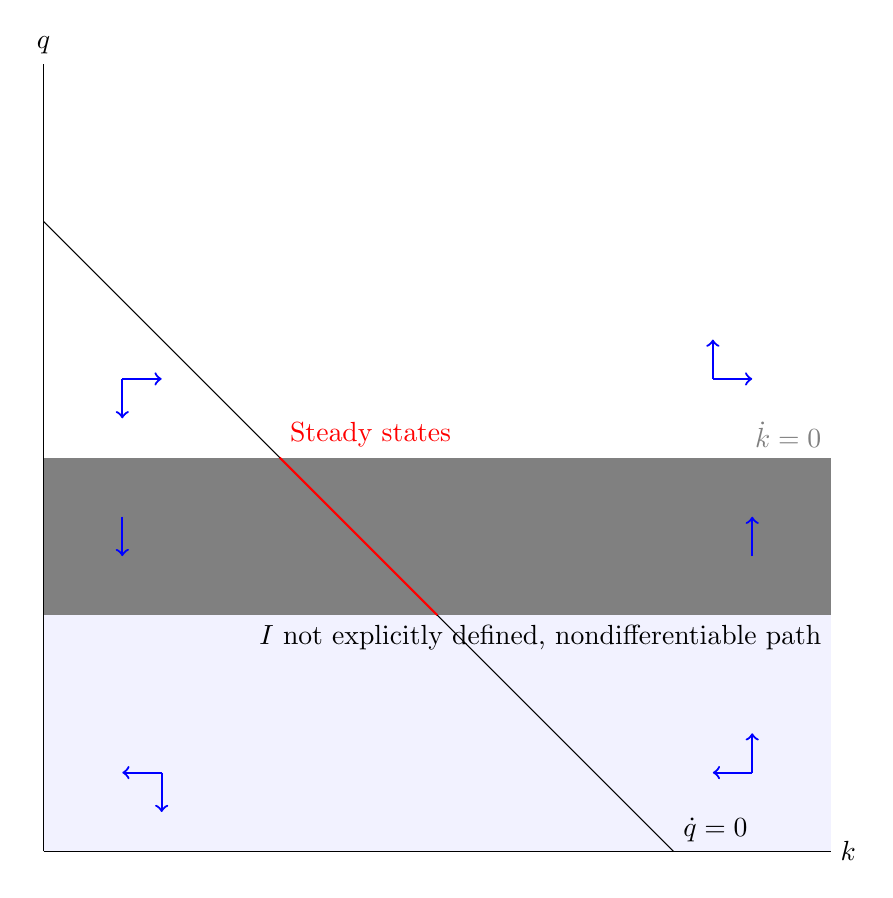
\begin{tikzpicture}
\draw (0,0) -- (10,0) node[anchor=west] {$k$};
\draw (0,0) -- (0,10) node[anchor=south] {$q$};
\fill [gray] (0,3) rectangle (10,5) node[anchor=south east] {$\dot{k} = 0$};
\fill [blue!5] (0,0) rectangle (10,3) node[anchor=north east, black] {$I$ not explicitly defined, nondifferentiable path};
\draw (0,8) -- (8,0) node[anchor=south west] {$\dot{q} = 0$};
\draw [thick, red] (5,3) -- (3,5) node[anchor=south west] {Steady states};
\draw [->, blue, thick] (1.5,1) -- (1,1);
\draw [->, blue, thick] (1.5,1) -- (1.5,0.5);
\draw [->, blue, thick] (1,6) -- (1.5,6);
\draw [->, blue, thick] (1,6) -- (1,5.5);
\draw [->, blue, thick] (1,4.25) -- (1,3.75);
\draw [->, blue, thick] (9,1) -- (8.5,1);
\draw [->, blue, thick] (9,1) -- (9,1.5);
\draw [->, blue, thick] (9,3.75) -- (9,4.25);
\draw [->, blue, thick] (8.5,6) -- (9,6);
\draw [->, blue, thick] (8.5,6) -- (8.5,6.5);
\end{tikzpicture}

\problempart{(5)}
If $k = a - rp^k(1-\omega)$, then $\frac{a-k}{rp^k} = 1-\omega = q$. Increasing $a$ shifts the $\dot{q} = 0$ line up. If the new $a'$ is such that
\[ \frac{a' - (a - rp^k(1-\omega))}{rp^k} > 1 \]
\[ a' - a > rp^k\omega \]
Then we jump to the regime above the inaction band and under the $\dot{q} = 0$ line, and capital increases to a new steady state. However, if $0 < a' - a < rp^k \omega$, then only the level of $q$ jumps up to a new steady state, and the firm makes no changes in capital. The adjustment costs add this friction to investment; due to the inaction region, the firm does not respond to this positive shock in productivity.
\problem{3}
See code. The plot of $V(K)$ is below

\begin{center}
\includegraphics[width=12cm]{ps2fig2}
\end{center}

The plot of $I(V')$ is below ($V' =$ marginal $q$)

\begin{center}
\includegraphics[width=12cm]{ps2fig3}
\end{center}


\end{document}
	% line of code telling latex that your document is ending. If you leave this out, you'll get an error
